\section{Ablations: the choice of \texorpdfstring{$f$}{f} and the orthonormality penalty}\label{sec:ablations}

The compact ablations vary one hyperparameter of each family on the finite four-rooms maze with goal $(5,5)$, the goal farthest from the start, with the seeds $0$, $1$, $2$ (\cref{tab:ablation,fig:ablation}).
The base runs are the core runs of that goal, reused by identifier; everything else in the protocol is unchanged.
One goal, one layout and three seeds make these ablations descriptive: they show what happened in these runs, not a ranking that would hold elsewhere.

\begin{table}[ht]
\centering\small
\caption{Compact ablations, finite four rooms, goal $(5,5)$, last checkpoint (mean $\pm$ SD over 3 seeds), with the first checkpoint at which each seed met the operational thresholds. The \fPG{} (JS), \ERFB{} and \DMFB{} rows are the core runs.}\label{tab:ablation}
\resizebox{\textwidth}{!}{% GENERATED by report/verify/make_tables.py from the saved run files (runs/jobs/*).
% Compact ablations, finite four rooms, goal (5,5): final held-out metrics (mean +/- SD, seeds 0-2) and first checkpoint meeting the thresholds per seed.
% Do not edit by hand: rerun  python3 report/verify/verify_results.py

\begin{tabular}{@{}lccccl@{}}
\toprule
method & JS (nats) & success & gap to $V^\star_H$ & $\JS^{\SA}$ (nats) & first reached (seeds 0, 1, 2)\\
\midrule
\fPG{} (JS) & $0.015\pm0.005$ & $1.000\pm0.000$ & $1.44\pm0.34$ & $0.048\pm0.019$ & 30k, 20k, 20k (transitions)\\
\fPG{} ($\KL(d\Vert q)$) & $0.012\pm0.005$ & $0.999\pm0.001$ & $1.72\pm0.44$ & $0.044\pm0.013$ & 30k, 30k, 30k (transitions)\\
\fPG{} ($\KL(q\Vert d)$) & $0.061\pm0.009$ & $0.998\pm0.002$ & $4.37\pm1.09$ & $0.146\pm0.044$ & 40k, 50k, 40k (transitions)\\
\midrule
\ERFB & $0.348\pm0.109$ & $0.772\pm0.196$ & $10.25\pm1.78$ & $0.425\pm0.085$ & --, --, -- (FB updates)\\
\ERFB, no orth. & $0.358\pm0.044$ & $0.965\pm0.017$ & $11.10\pm0.29$ & $0.490\pm0.039$ & --, --, -- (FB updates)\\
\DMFB & $0.476\pm0.204$ & $0.327\pm0.540$ & $11.38\pm1.64$ & $0.550\pm0.183$ & --, 5k, -- (FB updates)\\
\DMFB, no orth. & $0.467\pm0.067$ & $0.476\pm0.113$ & $11.85\pm0.26$ & $0.568\pm0.048$ & --, --, -- (FB updates)\\
\bottomrule
\end{tabular}
}
\end{table}

\begin{figure}[ht]
\centering
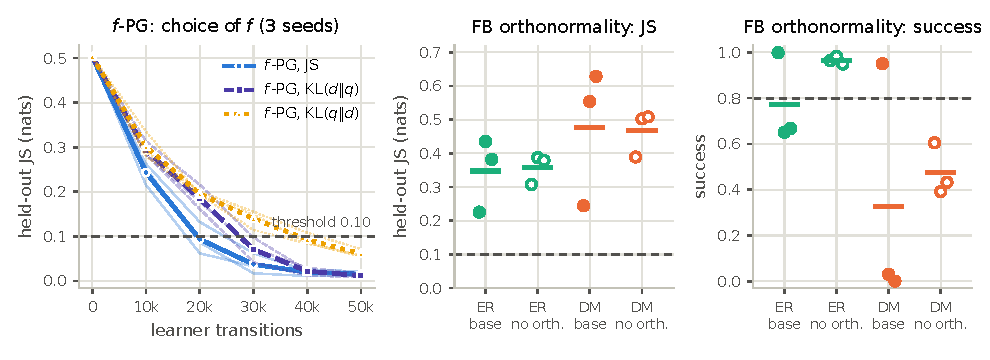
\includegraphics[width=\textwidth]{figures/fig_ablation.pdf}
\caption{Ablations (four rooms, goal $(5,5)$). Left: $f$-PG held-out divergence for three generators $f$ (thin lines: seeds; thick: mean). Middle and right: final \ERFB{} and \DMFB{} divergence and success with and without the orthonormality penalty (dots: seeds, open dots without the penalty; bars: means).}\label{fig:ablation}
\end{figure}

\subsection{The generator \texorpdfstring{$f$}{f} of \texorpdfstring{$f$}{f}-PG}

The three generators of \cref{sec:m-choice-f} were run with the same smoothing $\varepsilon=0.01$, the same initialization and first batch per seed, and the learning rate $0.3$ tuned for $\JS$; the $\KL$ runs were not tuned.
All nine runs meet the thresholds at the end of the budget, and the held-out divergence is the same $\JS(d^+_{\pi,H},q_E)$ for all of them, whatever $f$ was optimized.
\begin{itemize}[nosep]
\item $\KL(d\Vert q)$ behaves like $\JS$: final divergences $\vn{s13.kldq.js.lo}{0.0085}$ to $\vn{s13.kldq.js.hi}{0.0169}$ nats against $\vn{s13.js.js.lo}{0.0121}$ to $\vn{s13.js.js.hi}{0.0212}$, thresholds first met at the $\vn{s13.kldq.first30}{30{,}000}$-transition checkpoint in all three seeds (against $\vn{s13.js.first.lo}{20{,}000}$ to $\vn{s13.js.first.hi}{30{,}000}$), and similar returns ($\vn{s13.kldq.ret}{10.64}$ against $\vn{s13.js.ret}{10.92}$ on average).
\item $\KL(q\Vert d)$ is slower and ends further from the expert: thresholds first met at the $\vn{s09.klqd.first.lo}{40{,}000}$- to $\vn{s09.klqd.first.hi}{50{,}000}$-transition checkpoints, final divergences $\vn{s13.klqd.js.lo}{0.055}$ to $\vn{s13.klqd.js.hi}{0.071}$ nats, a mean return of $\vn{s13.klqd.ret}{7.99}$ (gap $\vn{s13.klqd.gap}{4.37}$ against $\vn{s13.js.gap}{1.44}$ for $\JS$), and a final state in the goal with probability $\vn{s13.klqd.fig}{0.82}$ against $\vn{s13.js.fig}{0.89}$. Its policies stay more stochastic (mean entropy $\vn{s13.klqd.ent}{0.38}$ nats on visited states, against $\vn{s13.js.ent}{0.12}$ for $\JS$ and $\vn{s13.kldq.ent}{0.16}$ for $\KL(d\Vert q)$), and their state--action divergence is \vn{s13.ratio}{three} times larger ($\vn{s13.klqd.jssa}{0.146}$ against $\vn{s13.js.jssa}{0.048}$).
\end{itemize}
The last observations agree with the shape of the signal (\cref{sec:m-choice-f}): $f'(v)=-1/v$ pushes hard towards under-visited expert cells and barely penalizes extra mass elsewhere, so a spread-out policy is cheap under $\KL(q\Vert d)$.
They cannot be separated from the learning rate: Adam makes the update roughly insensitive to the overall scale of the signal, but not to its shape, and the rate was tuned for $\JS$ only.
For $f$-IRL the same correspondence between $f$ and the per-state weight holds (\cref{prop:m-firl-fpg}), but nothing was run.

\subsection{The orthonormality penalty of FB}

Without the penalty, the backward Gram matrix drifts far from the identity (\cref{tab:fbdiag}): $\lambda_{\min}(\hat G_B)$ falls to $\vn{s13.noorth.lmin.lo}{0.05}$--$\vn{s13.noorth.lmin.hi}{0.19}$ and $\lambda_{\max}$ rises to $\vn{s13.noorth.lmax.lo}{118}$--$\vn{s13.noorth.lmax.hi}{146}$, against $\vn{s13.base.lmin.lo}{0.95}$--$\vn{s13.base.lmin.hi}{0.96}$ and $\vn{s13.base.lmax.lo}{2.3}$--$\vn{s13.base.lmax.hi}{2.7}$ with it, and $\lVert z_{ER}\rVert$ grows from $\vn{s13.base.erz.lo}{2.6}$--$\vn{s13.base.erz.hi}{2.9}$ to $\vn{s13.noorth.erz.lo}{13.8}$--$\vn{s13.noorth.erz.hi}{17.2}$ before projection.
The model is not worse by the oracle's measures: its sup-norm total-variation error is $\vn{s13.noorth.tv.lo}{21.7}$ to $\vn{s13.noorth.tv.hi}{44.8}$ (against $\vn{s13.base.tv.lo}{36.9}$ to $\vn{s13.base.tv.hi}{53.9}$) and its largest action-value error $\vn{s13.noorth.q.lo}{1.6}$ to $\vn{s13.noorth.q.hi}{6.2}$ (against $\vn{s13.base.q.lo}{2.7}$ to $\vn{s13.base.q.hi}{12.3}$).
But its policies are almost uniform: their entropy at the \DMFB{} start states is $\vn{s13.noorth.ent.lo}{1.30}$ to $\vn{s13.noorth.ent.hi}{1.44}$ nats (against $\vn{s13.base.ent.lo}{0.25}$ to $\vn{s13.base.ent.hi}{0.72}$, and $\log5\approx\vn{const.log5}{1.61}$).
This is consistent with the gauge freedom of the factorization: $(F,B)\mapsto(C^{-\top}F,CB)$ leaves the model's successor measures $F^\top B\nu$ unchanged but changes the scores $F^\top z$ that define $\pi_z$ at a fixed latent radius (\cref{prop:m-fb-softmax}(d)); without the penalty nothing fixes this gauge.

The imitation outcome changes less than the model.
No run, with or without the penalty, meets the thresholds at the end of the budget.
\ERFB{} without the penalty reaches the goal more often (success $\vn{s13.noorth.er.succ.lo}{0.95}$ to $\vn{s13.noorth.er.succ.hi}{0.98}$, against $\vn{s13.base.er.succ.lo}{0.65}$ to $\vn{s13.base.er.succ.hi}{1.00}$) at a similar divergence ($\vn{s13.noorth.er.js}{0.358}$ against $\vn{s13.base.er.js}{0.348}$ nats on average); this is consistent with nearly uniform policies that diffuse to the goal without staying there (final state in the goal with probability $\vn{s13.noorth.er.fig}{0.13}$ on average, against $\vn{s13.base.er.fig}{0.12}$).
\DMFB{} has a similar mean divergence with and without the penalty ($\vn{s13.noorth.dm.js}{0.467}$ against $\vn{s13.base.dm.js}{0.476}$ nats) but a much smaller spread across seeds.
The penalty is therefore not what limits FB imitation in these runs.
What differed with and without it is the conditioning of $\hat G_B$ and the entropy of the policies, as reported above: with the penalty, $\hat G_B$ was well conditioned and the policies were far from uniform.
This is an observation on three seeds of one finite task, not a guarantee: the penalty is soft and only encourages conditioning and scale control (\cref{prop:m-fb-orth}(c)), and with the penalty on, the continuous Gram matrices were nearly singular ($\lambda_{\min}$ between $\vn{s12.lmin.lo}{1.7\times10^{-5}}$ and $\vn{s12.lmin.hi}{4.2\times10^{-5}}$, \cref{sec:results-continuous}).
